% Saberes básicos (LOMLOE) asociados a esta unidad
%
% Bloque A. Las destrezas científicas básicas
%   - Uso del lenguaje científico y de las unidades del Sistema Internacional (SI):
%     la unidad se trabaja con el julio y sus múltiplos/submúltiplos, además de otras
%     unidades de energía de uso habitual (caloría, kWh, tep), reforzando el manejo
%     correcto de magnitudes y unidades ya introducido en la Unidad 1.
%
% Bloque C. La energía
%   - Formulación de cuestiones e hipótesis sobre la energía, sus propiedades y
%     manifestaciones como causa de todos los procesos de cambio: se define la energía,
%     sus formas (cinética, potencial, térmica, eléctrica, radiante, química, nuclear)
%     y sus propiedades (se transfiere, se almacena, se transporta, se transforma,
%     se degrada y se conserva).
%   - Diseño y comprobación experimental de hipótesis sobre el uso doméstico e industrial
%     de la energía y las transformaciones entre sus distintas formas: se analizan cadenas
%     de transformación energética en aparatos cotidianos (linterna, secador, aerogenerador,
%     hervidor, panel solar) y el concepto de degradación/rendimiento.
%   - Elaboración fundamentada de hipótesis sobre el medio ambiente y la sostenibilidad a
%     partir de las diferencias entre fuentes renovables y no renovables. Valoración de la
%     producción de energía eólica en Castilla-La Mancha: se dedica un apartado específico
%     a la energía eólica en la región, con sus ventajas y sus impactos.
%   - Efectos del calor sobre la materia: se incorpora un apartado sobre el calor específico
%     y la dilatación térmica, con ejemplos y aplicaciones cotidianas (juntas de dilatación,
%     termómetros de líquido, clima costero frente a clima de interior).
%   - Naturaleza eléctrica de la materia: electrización de los cuerpos, circuitos eléctricos
%     y obtención de energía eléctrica: se desarrollan la ley de Ohm y los circuitos en serie
%     y en paralelo, junto con el ahorro energético y la conservación sostenible del medio
%     ambiente, ya tratados en la unidad.

\spacing{1.3}
\raggedbottom % pages with large figures end where the text ends (no stretched gaps between boxes)

\section{¿Qué es la energía?}

\begin{definition}[Energía]
    Magnitud física que mide la capacidad que tiene un cuerpo para producir cambios en sí mismo o en otros cuerpos.
\end{definition}

Siempre que una persona, una máquina o cualquier otro objeto hace algo, gasta energía, y tiene que conseguir más para seguir funcionando.

\begin{didyouknow}
    Tu cerebro gasta alrededor del 20\,\% de toda la energía que tu cuerpo obtiene de los alimentos, ¡aunque solo supone un 2\,\% de tu masa corporal!
\end{didyouknow}

\subsection{¿Cómo se mide la energía?}

En el SI, la energía se mide en \textbf{julios} (J); también se usa mucho el kilojulio (\qty{1}{\kj} = \qty{1000}{\joule}). Además, hay otras unidades que se emplean en ámbitos concretos:

\begin{itemize}
    \item \negsubro{Caloría} (cal): cantidad de calor necesaria para elevar \qty{1}{\celsius} la temperatura de \qty{1}{\g} de agua. \(\qty{1}{\calorie} = \qty{4.18}{\joule}\). La energía de los alimentos se ha expresado tradicionalmente en Calorías (con C mayúscula): \(1 \text{ Caloría} = 1000 \text{ calorías} = \qty{1}{\kilo\calorie}\).
    \item \negsubro{Kilovatio hora} (kWh): se usa para medir la energía eléctrica; es la energía que consume un aparato de \qty{1}{\kW} funcionando durante una hora. \(\qty{1}{\kwh} = \qty{3.6e6}{\joule}\).
    \item \negsubro{Tonelada equivalente de petróleo} (tep): se usa en la industria del petróleo; es la energía que se obtiene al quemar \qty{1000}{\kg} de petróleo. \(1 \text{ tep} \approx \qty{4.187e10}{\joule}\).
\end{itemize}

\begin{figure}[H]
    \centering
    % [FIGURA ORIGINAL] \includegraphics[width=\textwidth]{Unit_9/energy_units}
    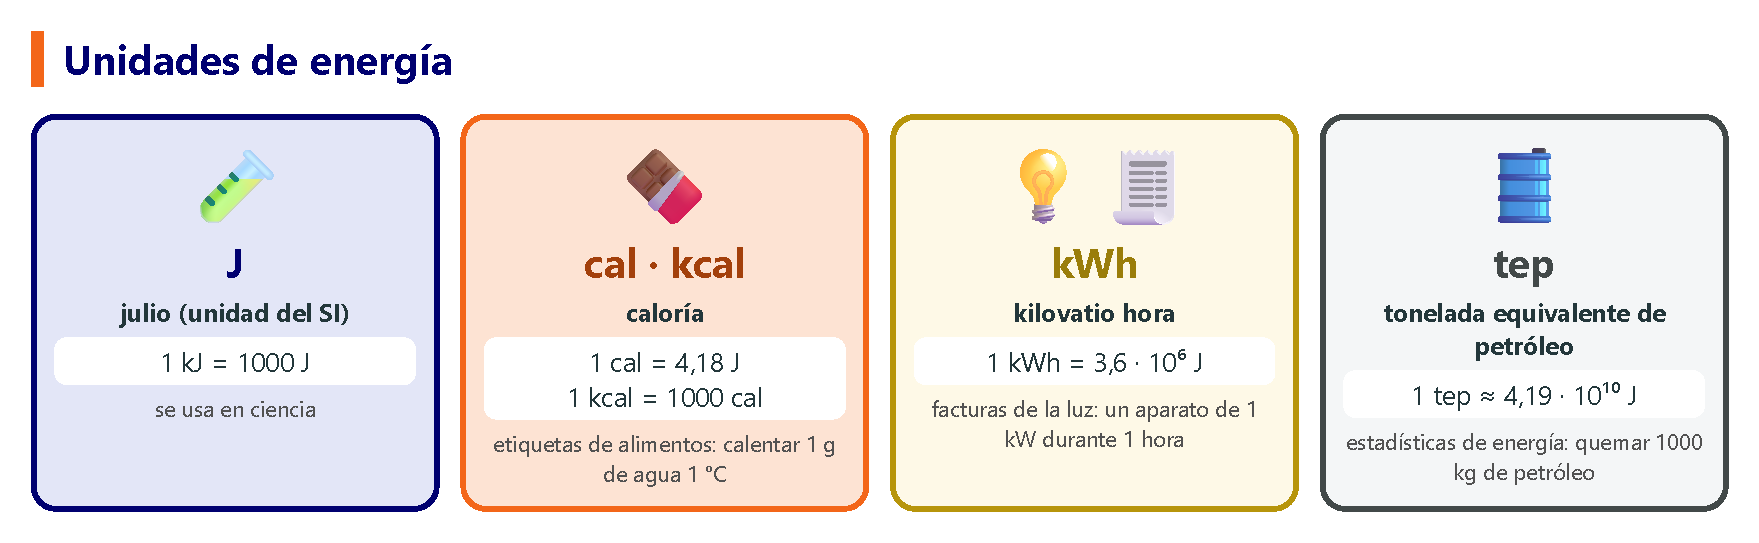
\includegraphics[width=\textwidth]{FigurasSVG/Unit_9_Energy/pdf/energy_units_es.pdf}
    \caption{Las unidades de energía más habituales y dónde las encontramos.}
    \label{fig:u9_energy_units}
\end{figure}

\begin{example}
    \textbf{Un balón cae de una canasta al suelo con una energía de \qty{18.2}{\joule}. Expresa esta cantidad en kJ, cal y kWh.}
    \begin{align*}
        \qty{18.2}{\joule} \cdot \dfrac{\qty{1}{\kilo\joule}}{\qty{1000}{\joule}} &= \textbf{\num{0.018} kJ} \\
        \qty{18.2}{\joule} \cdot \dfrac{\qty{1}{\calorie}}{\qty{4.18}{\joule}} &= \textbf{\num{4.35} cal} \\
        \qty{18.2}{\joule} \cdot \dfrac{\qty{1}{\kwh}}{\qty{3.6e6}{\joule}} &\approx \textbf{\num{5.06}} \times \textbf{10}^{\textbf{-6}} \textbf{ kWh}
    \end{align*}
\end{example}

\begin{exercise}
    Para preparar una taza de té se calienta agua de \qty{20}{\celsius} a \qty{100}{\celsius} en un microondas que le aporta \qty{83860}{\joule}.
    \begin{enumerate}[label=\letraminuscula]
        \item ¿Cuántas calorías son?
        \item ¿Cuántos kWh son?
    \end{enumerate}
    \begin{solu}
        \begin{enumerate}[label=\alph*)]
            \item \(\qty{83860}{\joule} \cdot \dfrac{\qty{1}{\calorie}}{\qty{4.18}{\joule}} \approx \num{20062}\) cal.
            \item \(\qty{83860}{\joule} \cdot \dfrac{\qty{1}{\kwh}}{\qty{3.6e6}{\joule}} \approx \num{0.0233}\) kWh.
        \end{enumerate}
    \end{solu}
\end{exercise}

\begin{exercise}
    El contenido energético de \qty{100}{\g} de galletas es de unas \qty{350}{\kilo\calorie}. Expresa esta cantidad en julios.
    \begin{solu}
        \(\qty{350}{\kilo\calorie} = \qty{350000}{\calorie}\); \(\qty{350000}{\calorie} \cdot \qty{4.18}{\joule\per\calorie} \approx \qty{1463000}{\joule} \approx \qty{1.46}{\mega\joule}\).
    \end{solu}
\end{exercise}

\begin{exercise}
    Una lavadora gasta \qty{1.1}{\kwh} de energía eléctrica en un lavado completo.
    \begin{enumerate}[label=\letraminuscula]
        \item Pasa esta energía a julios.
        \item Pasa esta energía a calorías.
    \end{enumerate}
    \begin{solu}
        \begin{enumerate}[label=\alph*)]
            \item \(\qty{1.1}{\kwh} \cdot \qty{3.6e6}{\joule\per\kwh} = \qty{3960000}{\joule} \approx \qty{3.96}{\mega\joule}\).
            \item \(\qty{3960000}{\joule} \cdot \dfrac{\qty{1}{\calorie}}{\qty{4.18}{\joule}} \approx \num{947368}\) cal \(\approx \num{947.4}\) kcal.
        \end{enumerate}
    \end{solu}
\end{exercise}

\begin{exercise}
    Una instalación de paneles solares produce \qty{2.5}{\mega\joule} de energía en un día. Expresa esta cantidad en kWh y en kcal.
    \begin{solu}
        \(\qty{2.5}{\mega\joule} = \qty{2500000}{\joule}\). \\
        En kWh: \(\qty{2500000}{\joule} \cdot \dfrac{\qty{1}{\kwh}}{\qty{3.6e6}{\joule}} \approx \textbf{\num{0.694} kWh}\). \\
        En kcal: \(\qty{2500000}{\joule} \cdot \dfrac{\qty{1}{\calorie}}{\qty{4.18}{\joule}} \approx \num{598086}\) cal \(\approx \textbf{\num{598.1} kcal}\).
    \end{solu}
\end{exercise}

%----------------------------------------------------------------------------------------

\section{Formas de energía}

\begin{figure}[H]
    \centering
    % [FIGURA ORIGINAL] \includegraphics[width=\textwidth]{Unit_9/forms_energy}
    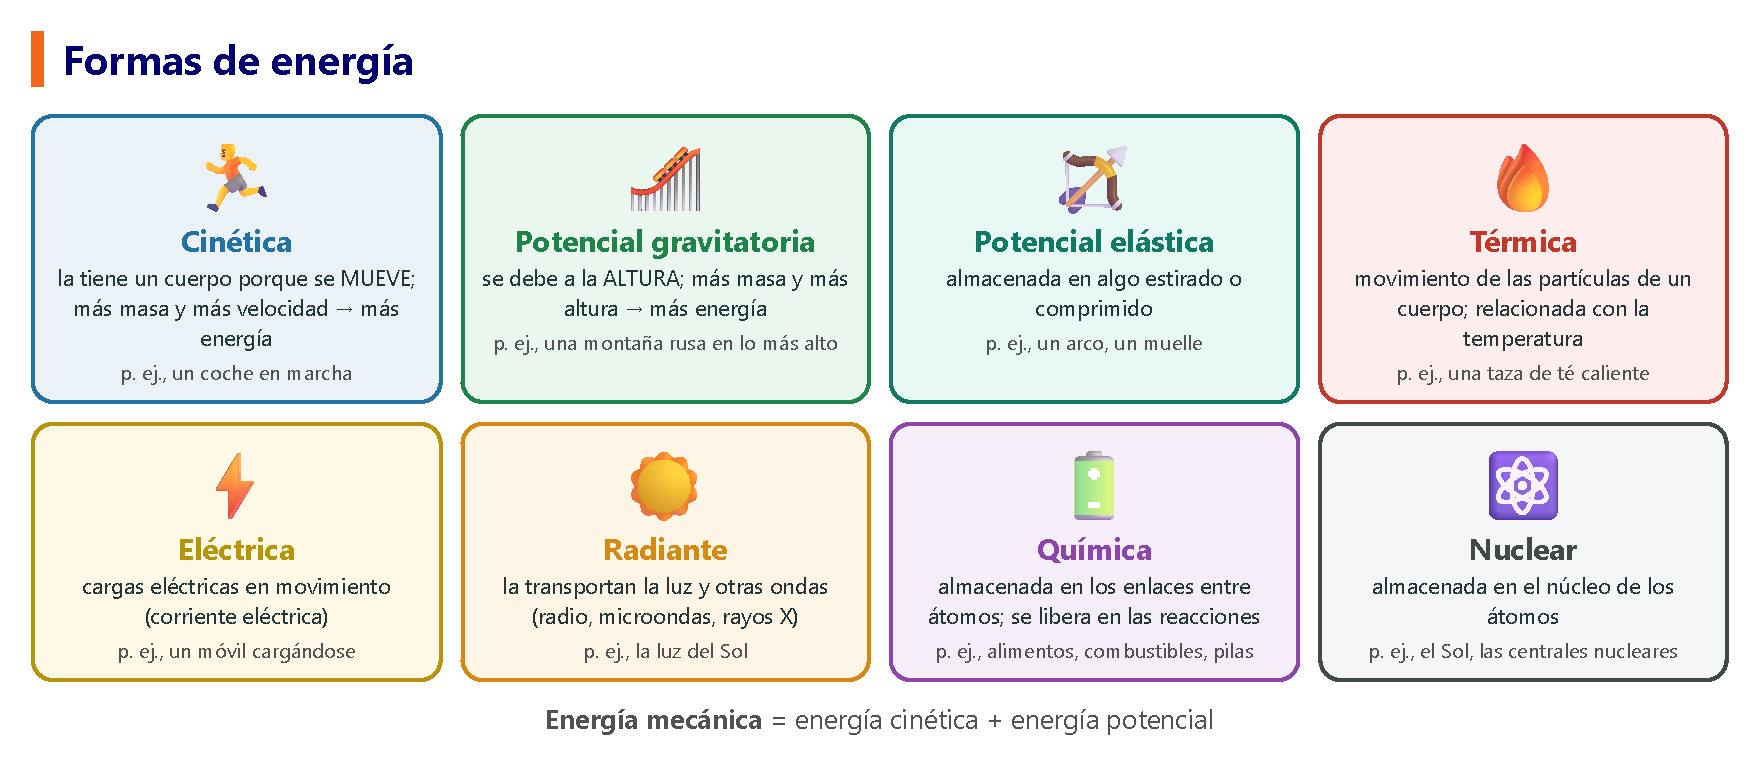
\includegraphics[width=\textwidth]{FigurasSVG/Unit_9_Energy/pdf/forms_energy_es.pdf}
    \caption{Las formas de energía.}
    \label{fig:u9_forms_energy}
\end{figure}

\begin{impt}
    \negsubro{Fusión nuclear y fisión nuclear}:
    \begin{itemize}
        \item \textbf{Fusión nuclear}: átomos ligeros se unen para formar átomos más grandes y se libera energía (es lo que ocurre en el Sol y en las demás estrellas).
        \item \textbf{Fisión nuclear}: átomos pesados se rompen en átomos más pequeños y se libera energía (es lo que ocurre en las centrales nucleares).
    \end{itemize}
\end{impt}

\begin{figure}[H]
    \centering
    % [FIGURA ORIGINAL] \includegraphics[width=\textwidth]{Unit_9/fusion_fission}
    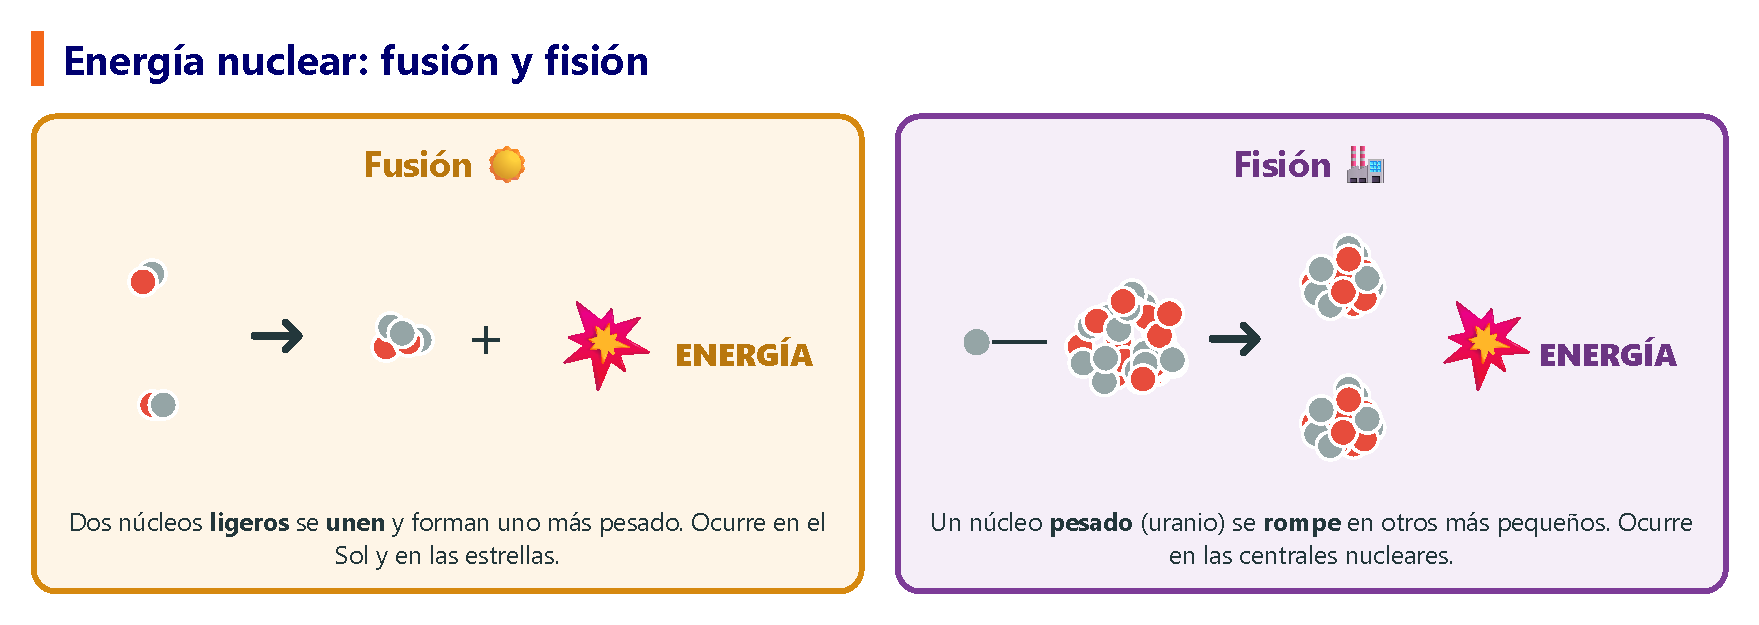
\includegraphics[width=\textwidth]{FigurasSVG/Unit_9_Energy/pdf/fusion_fission_es.pdf}
    \caption{Fusión nuclear y fisión nuclear.}
    \label{fig:u9_fusion_fission}
\end{figure}

\begin{didyouknow}
    Cada segundo, el Sol convierte en energía unos 4 millones de toneladas de materia mediante la fusión nuclear. Lleva haciéndolo \num{4600} millones de años, ¡y aún le queda combustible para unos \num{5000} millones de años más!
\end{didyouknow}

\begin{example}
    Si un camión y un coche van a la misma velocidad, el camión tiene más \textbf{energía cinética} porque tiene más masa. Un mismo coche tiene más energía cinética cuanto más deprisa va. Una pelota tiene más \textbf{energía potencial gravitatoria} cuanto más alta está y cuanta más masa tiene. Un arco tensado tiene más \textbf{energía potencial elástica} cuanto más se tensa.
\end{example}

\begin{exercise}
    Indica qué forma o formas de energía intervienen en cada situación: a) una bicicleta en movimiento; b) un secador que calienta y expulsa aire; c) una nadadora que se tira a la piscina; d) una taza de té caliente; e) una radiografía; f) un tirachinas tensado.
    \begin{solu}
        \begin{enumerate}[label=\alph*)]
            \item Energía cinética (mecánica).
            \item Energía eléctrica (que se transforma en energía térmica y en energía cinética del aire).
            \item Energía cinética y energía potencial gravitatoria.
            \item Energía térmica.
            \item Energía radiante.
            \item Energía potencial elástica.
        \end{enumerate}
    \end{solu}
\end{exercise}

\begin{exercise}
    ¿Qué tipos de energía intervienen cuando usamos un teléfono móvil y qué transformaciones se producen?
    \begin{solu}
        La batería almacena \textbf{energía química}; al usar el móvil, esta se transforma en \textbf{energía eléctrica}, que el teléfono transforma a su vez en \textbf{energía radiante} (la luz de la pantalla), \textbf{energía térmica} (el móvil se calienta) y, si hacemos una llamada, en energía \textbf{sonora} (mecánica) en el altavoz.
    \end{solu}
\end{exercise}

\begin{exercise}
    Clasifica la principal transformación de energía que se produce en cada caso (antes \(\to\) después): a) una cocina solar; b) un coche de juguete de cuerda; c) una cerilla encendida; d) una central nuclear.
    \begin{solu}
        \begin{enumerate}[label=\alph*)]
            \item Energía radiante (luz del Sol) \(\to\) energía térmica.
            \item Energía potencial elástica (muelle con cuerda) \(\to\) energía cinética.
            \item Energía química \(\to\) energía térmica \(+\) energía radiante (luz).
            \item Energía nuclear \(\to\) energía térmica \(\to\) energía eléctrica.
        \end{enumerate}
    \end{solu}
\end{exercise}

%----------------------------------------------------------------------------------------

\section{Propiedades de la energía}

\begin{figure}[H]
    \centering
    % [FIGURA ORIGINAL] \includegraphics[width=\textwidth]{Unit_9/energy_properties}
    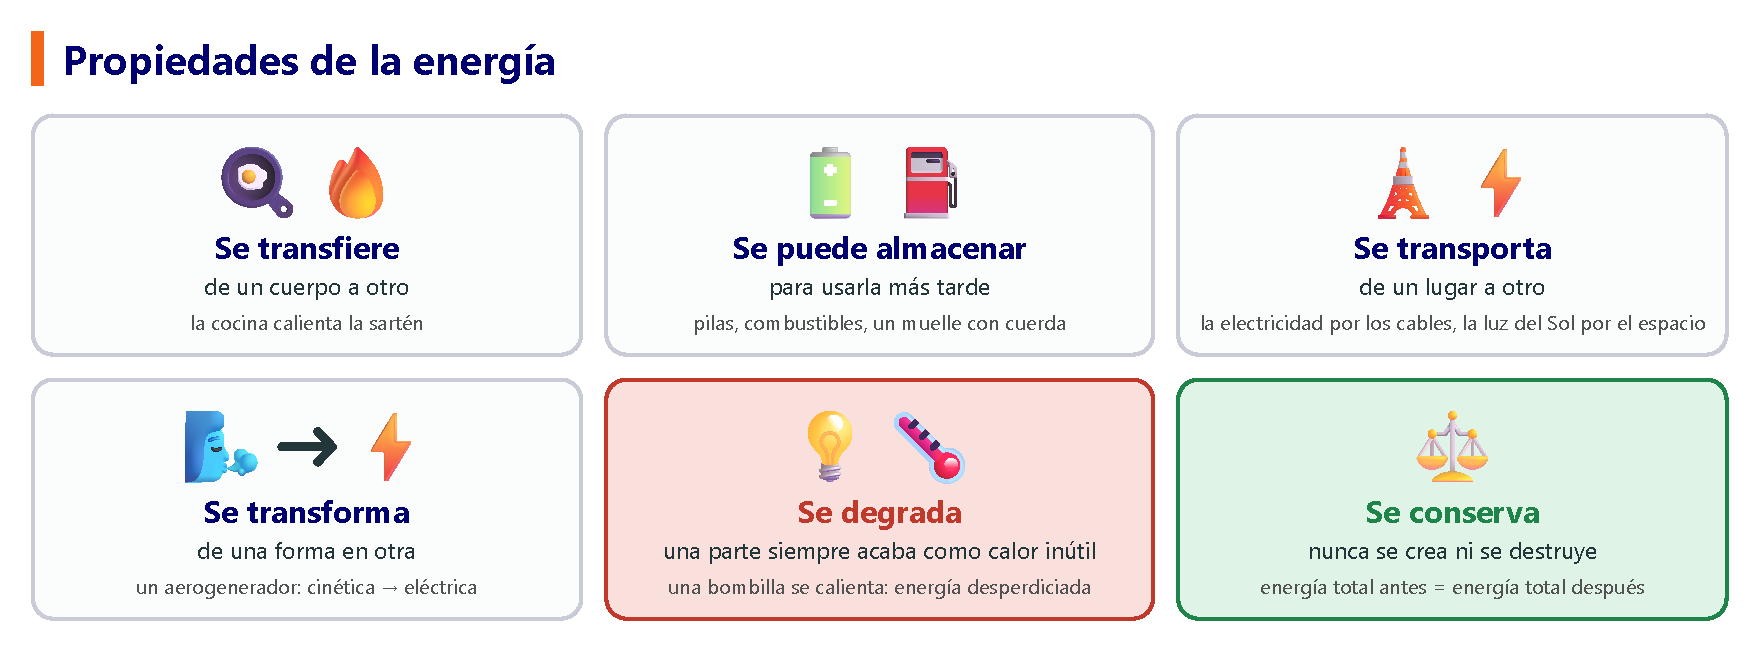
\includegraphics[width=\textwidth]{FigurasSVG/Unit_9_Energy/pdf/energy_properties_es.pdf}
    \caption{Las seis propiedades de la energía.}
    \label{fig:u9_energy_properties}
\end{figure}

\begin{example}
    \textbf{Cadena de transformaciones de la energía en una linterna}: energía química (pila) \(\to\) energía eléctrica \(\to\) energía radiante (luz) \(+\) energía térmica (degradada, calienta la linterna). La energía total transformada se conserva, pero solo la energía radiante es útil.
\end{example}

\begin{figure}[H]
    \centering
    % [FIGURA ORIGINAL] \includegraphics[width=\textwidth]{Unit_9/torch_chain}
    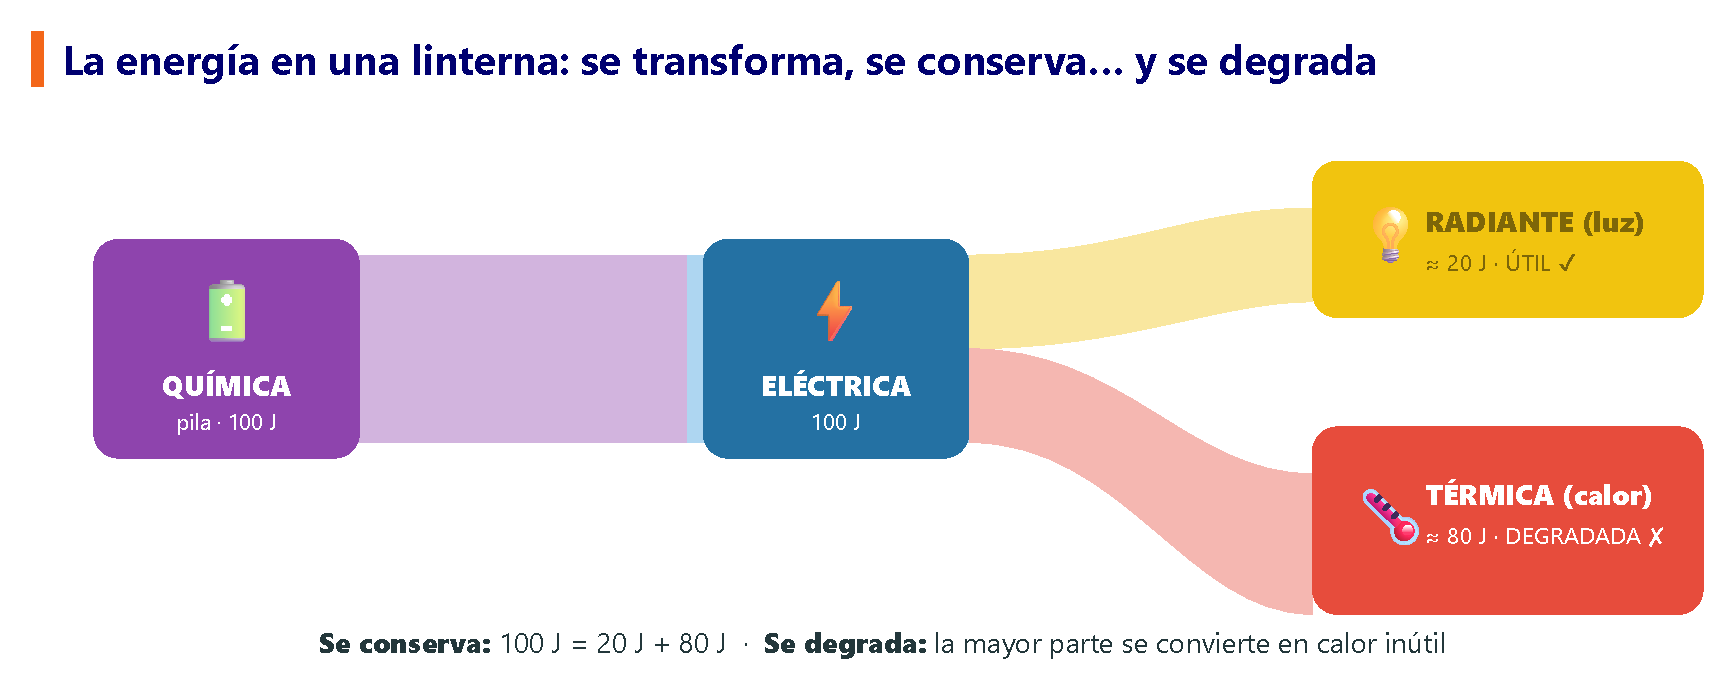
\includegraphics[width=\textwidth]{FigurasSVG/Unit_9_Energy/pdf/torch_chain_es.pdf}
    \caption{La energía en una linterna: la energía total se conserva, pero la mayor parte se degrada en forma de calor.}
    \label{fig:u9_torch_chain}
\end{figure}

\begin{exercise}
    Para cada aparato, escribe la cadena de transformaciones de la energía, desde la fuente de energía hasta la energía útil que se obtiene: a) un aerogenerador que produce electricidad; b) un hervidor eléctrico que pone el agua a hervir; c) un panel solar que calienta agua directamente (sin producir electricidad).
    \begin{solu}
        \begin{enumerate}[label=\alph*)]
            \item Energía cinética (viento) \(\to\) energía mecánica (giro de las palas y del generador) \(\to\) energía eléctrica.
            \item Energía eléctrica \(\to\) energía térmica (calienta el agua).
            \item Energía radiante (luz del Sol) \(\to\) energía térmica (calienta el agua directamente).
        \end{enumerate}
    \end{solu}
\end{exercise}

\begin{exercise}
    Dejamos caer una pelota desde cierta altura y bota varias veces, pero en cada bote llega más bajo que en el anterior. Explica por qué ocurre esto usando las propiedades de la energía, y di si se destruye energía.
    \begin{solu}
        En cada bote, parte de la energía mecánica de la pelota se \textbf{transforma} en energía térmica y en sonido, por el rozamiento con el aire y por la deformación al chocar con el suelo. Es una \textbf{degradación} de la energía: queda menos energía útil (mecánica) para el siguiente bote, y por eso cada vez sube menos. No se destruye energía: la energía total siempre se \textbf{conserva}; simplemente se transforma en formas menos útiles.
    \end{solu}
\end{exercise}

\subsection{Cómo intercambian energía los cuerpos}

\begin{itemize}
    \item \negsubro{En forma de calor}: los cuerpos que están a distinta temperatura intercambian energía hasta que alcanzan la misma temperatura (p.\ ej., el hielo, al fundirse, absorbe calor del aire).
    \item \negsubro{En forma de trabajo mecánico}: ocurre cuando una fuerza produce un movimiento (p.\ ej., tensar un arco o empujar un carro de la compra).
\end{itemize}

\begin{figure}[H]
    \centering
    % [FIGURA ORIGINAL] \includegraphics[width=\textwidth]{Unit_9/heat_work}
    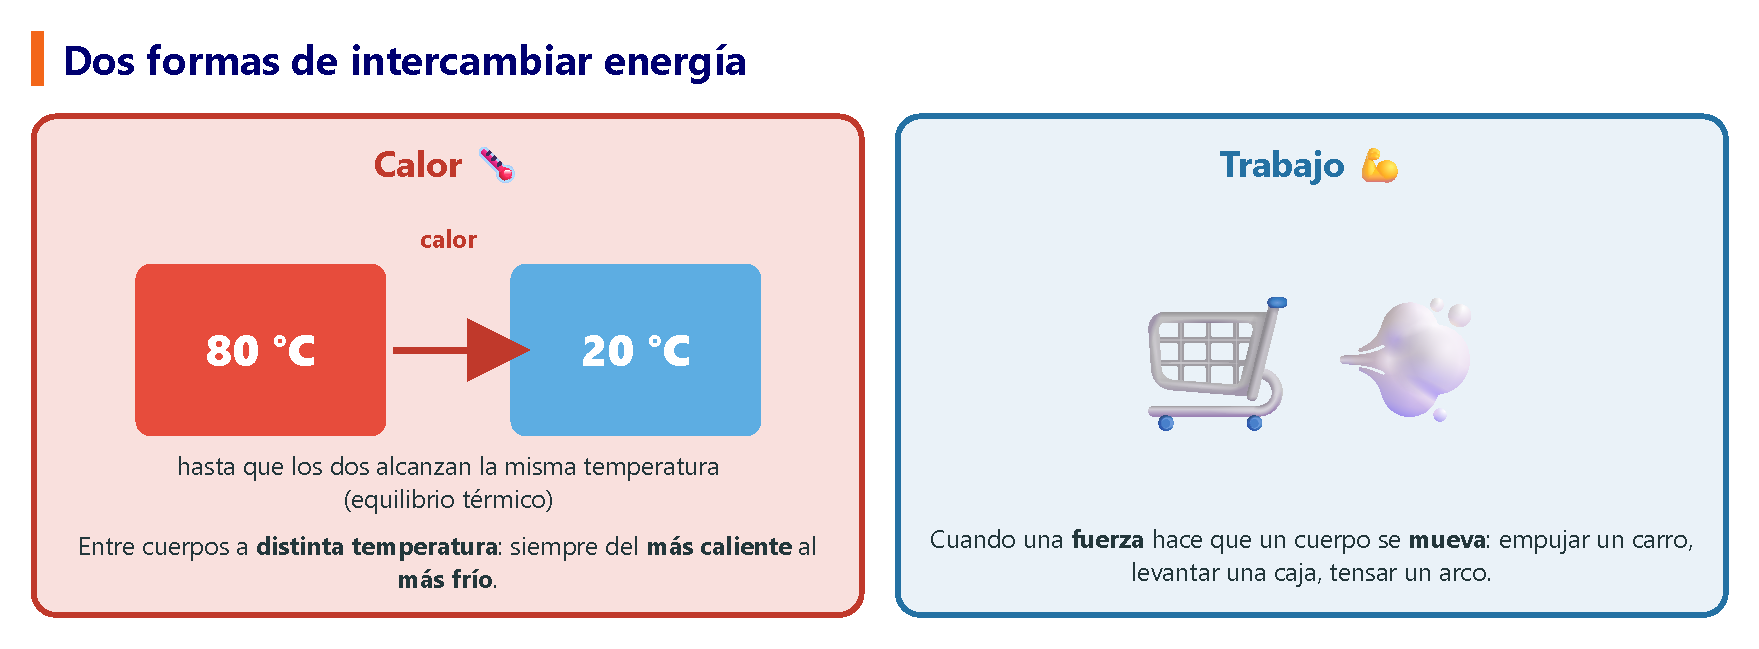
\includegraphics[width=\textwidth]{FigurasSVG/Unit_9_Energy/pdf/heat_work_es.pdf}
    \caption{Los cuerpos intercambian energía en forma de calor o de trabajo.}
    \label{fig:u9_heat_work}
\end{figure}

\begin{exercise}
    Identifica la propiedad de la energía que interviene en cada situación: a) al enchufar un secador, sale una corriente de aire; b) la batería de un móvil dura tres días; c) al meter una botella de agua en la nevera, se enfría; d) las bombillas que se calientan no son muy eficientes; e) los cables de alta tensión llevan la electricidad de un extremo a otro del país.
    \begin{solu}
        \begin{enumerate}[label=\alph*)]
            \item La energía se \textbf{transforma} (la eléctrica en cinética y térmica).
            \item La energía se \textbf{almacena} (energía química en la batería).
            \item La energía se \textbf{transfiere} en forma de calor (del agua al aire frío de la nevera).
            \item La energía se \textbf{degrada} (parte de la energía eléctrica se convierte en calor en lugar de en luz).
            \item La energía se \textbf{transporta}.
        \end{enumerate}
    \end{solu}
\end{exercise}

\begin{exercise}
    El rendimiento de una máquina es la relación entre la energía que queremos obtener de ella y la energía que consume. ¿Qué propiedad de la energía hace que el rendimiento de una máquina sea siempre menor del 100\,\%?
    \begin{solu}
        La \textbf{degradación de la energía}: cada vez que la energía se transforma, una parte se convierte en calor no aprovechable, así que una máquina nunca puede devolver como energía útil el 100\,\% de la energía que consume.
    \end{solu}
\end{exercise}

\begin{exercise}
    Dentro de una caja aislante se ponen en contacto dos bloques de metal, uno a \qty{80}{\celsius} y otro a \qty{20}{\celsius}. Describe qué le ocurre a la energía de cada bloque hasta que alcanzan el equilibrio térmico, e indica de qué forma se intercambia la energía.
    \begin{solu}
        El calor pasa del bloque más caliente (\qty{80}{\celsius}) al más frío (\qty{20}{\celsius}) hasta que los dos alcanzan la misma temperatura, intermedia entre ambas (equilibrio térmico). La energía se intercambia \textbf{en forma de calor}; no se realiza trabajo mecánico, ya que ninguno de los bloques se mueve.
    \end{solu}
\end{exercise}

\subsection{Efectos del calor sobre la materia}

\begin{definition}[Calor específico]
    Cantidad de calor necesaria para elevar \qty{1}{\celsius} la temperatura de \qty{1}{\kg} de una sustancia. Se representa con la letra \(c\) y su unidad en el SI es el \unit{\joule\per\kg\per\celsius}.
    \begin{equation*}
        Q = m \cdot c \cdot \Delta T
    \end{equation*}
\end{definition}

El agua tiene un calor específico muy alto, \(c_{\text{agua}} = \qty{4180}{\joule\per\kg\per\celsius}\) (equivale a \(\qty{1}{\calorie}/(\text{g} \cdot {}^{\circ}\text{C})\)): por eso el agua se calienta y se enfría más despacio que la mayoría de las sustancias, y por eso los lugares cercanos a la costa suelen tener un clima más suave que los que están lejos del mar.

\begin{figure}[H]
    \centering
    % [FIGURA ORIGINAL] \includegraphics[width=\textwidth]{Unit_9/specific_heat}
    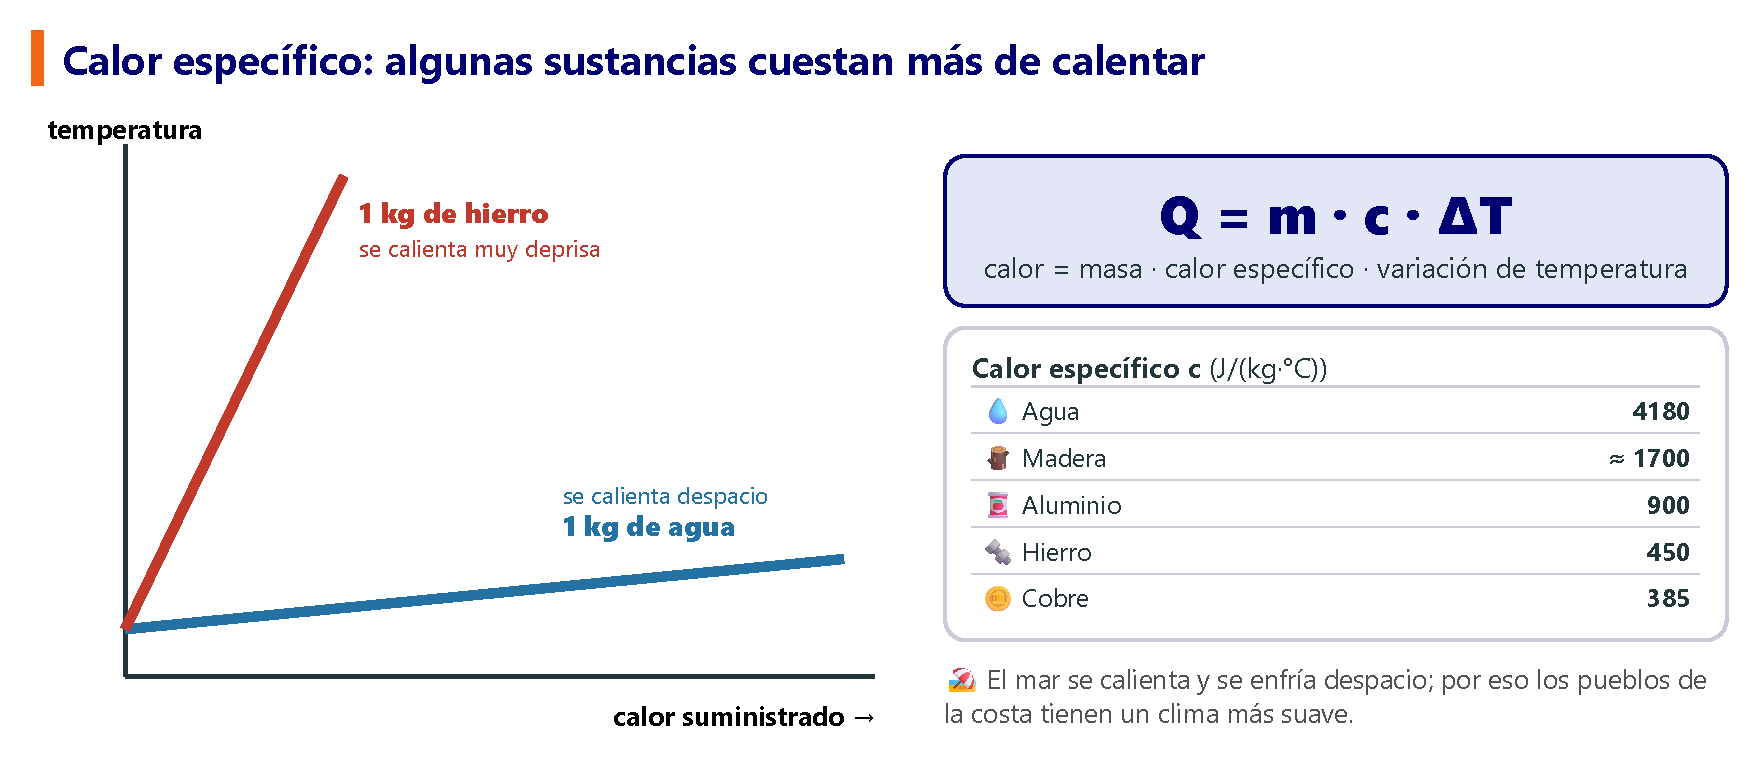
\includegraphics[width=\textwidth]{FigurasSVG/Unit_9_Energy/pdf/specific_heat_es.pdf}
    \caption{Con el mismo calor, el hierro se calienta mucho más que el agua: el agua tiene un calor específico muy alto.}
    \label{fig:u9_specific_heat}
\end{figure}

\begin{example}
    \textbf{¿Cuánto calor hace falta para elevar la temperatura de \qty{2}{\kg} de agua de \qty{18}{\celsius} a \qty{38}{\celsius}?}
    \begin{equation*}
        Q = m \cdot c \cdot \Delta T = \qty{2}{\kg} \cdot 4180 \dfrac{\text{J}}{\text{kg} \cdot {}^{\circ}\text{C}} \cdot (38 - 18)\ {}^{\circ}\text{C} = \textbf{\num{167200} J} \approx \textbf{\num{167.2} kJ}
    \end{equation*}
\end{example}

\begin{exercise}
    Calcula el calor necesario para elevar la temperatura de \qty{0.5}{\kg} de agua de \qty{15}{\celsius} a \qty{100}{\celsius} en un hervidor. Da el resultado en kJ y en kcal.
    \begin{solu}
        \(Q = \qty{0.5}{\kg} \cdot 4180 \dfrac{\text{J}}{\text{kg} \cdot {}^{\circ}\text{C}} \cdot (100-15)\ {}^{\circ}\text{C} = \qty{177650}{\joule} \approx \qty{177.65}{\kilo\joule}\). \\
        En kcal: \(\qty{177650}{\joule} \cdot \dfrac{\qty{1}{\calorie}}{\qty{4.18}{\joule}} \approx \qty{42500}{\calorie} \approx \textbf{\num{42.5} kcal}\).
    \end{solu}
\end{exercise}

\begin{exercise}
    Un bloque de \qty{1.5}{\kg} de un metal desconocido absorbe \qty{13500}{\joule} de calor y su temperatura sube de \qty{20}{\celsius} a \qty{45}{\celsius}. Calcula su calor específico.
    \begin{solu}
        A partir de \(Q = m \cdot c \cdot \Delta T\): \(c = \dfrac{Q}{m \cdot \Delta T} = \dfrac{\qty{13500}{\joule}}{\qty{1.5}{\kg} \cdot (45-20)\ {}^{\circ}\text{C}} = \dfrac{\num{13500}}{\num{37.5}} = \textbf{360}\ \unit{\joule\per\kg\per\celsius}\).
    \end{solu}
\end{exercise}

\begin{impt}
    \negsubro{Dilatación térmica}: la mayoría de las sustancias aumentan de volumen cuando sube su temperatura y lo disminuyen cuando baja: se \textbf{dilatan} al calentarse y se \textbf{contraen} al enfriarse. Los gases son los que más se dilatan, seguidos de los líquidos y, por último, de los sólidos.
\end{impt}

\begin{figure}[H]
    \centering
    % [FIGURA ORIGINAL] \includegraphics[width=\textwidth]{Unit_9/thermal_expansion}
    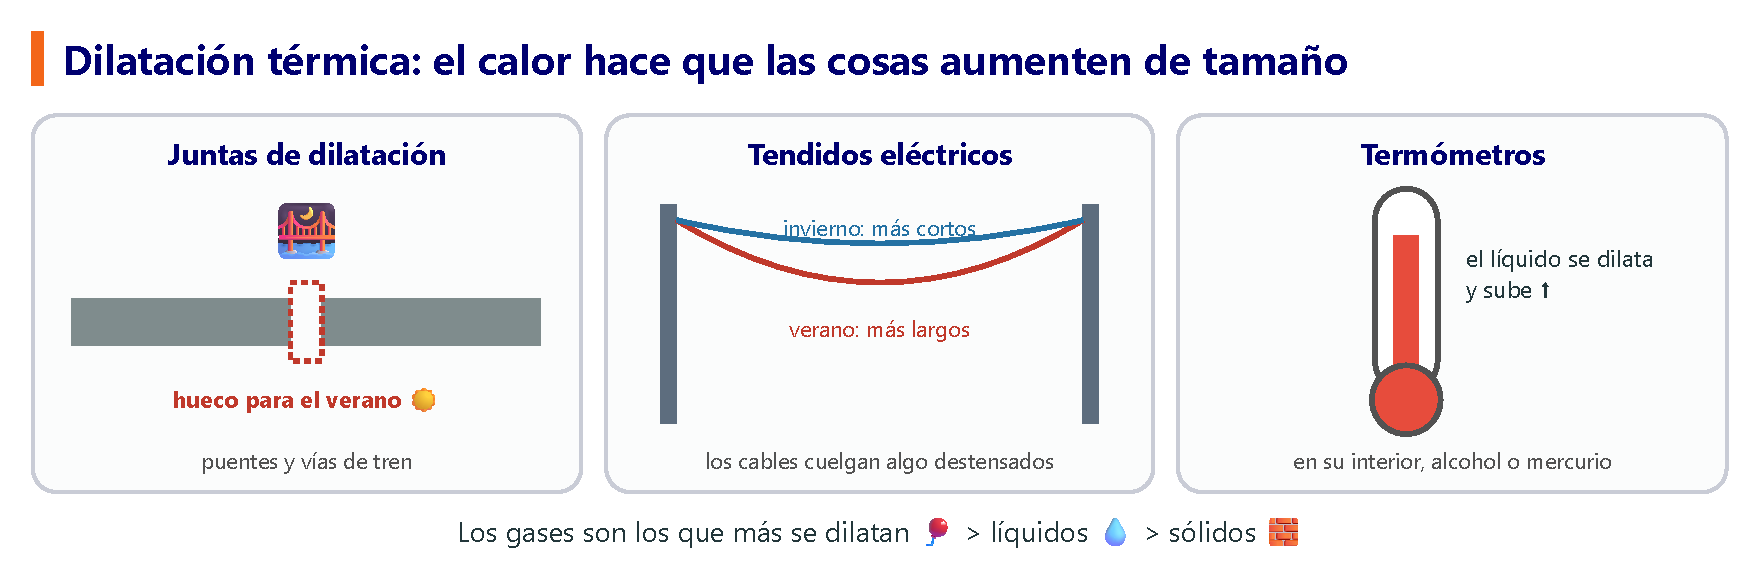
\includegraphics[width=\textwidth]{FigurasSVG/Unit_9_Energy/pdf/thermal_expansion_es.pdf}
    \caption{Ejemplos cotidianos de dilatación térmica.}
    \label{fig:u9_thermal_expansion}
\end{figure}

\begin{exercise}
    Explica por qué los cables de los tendidos eléctricos se cuelgan algo destensados entre las torres, en lugar de dejarlos muy tirantes.
    \begin{solu}
        En verano, los cables metálicos se calientan y se \textbf{dilatan}, es decir, se alargan un poco; al estar algo destensados, pueden hacerlo sin romperse ni dañarse. En invierno, los cables se enfrían y vuelven a contraerse.
    \end{solu}
\end{exercise}

\begin{exercise}
    Indica qué se dilata más al calentarse, los sólidos, los líquidos o los gases, y explica por qué un globo aerostático sube cuando se calienta el aire de su interior.
    \begin{solu}
        Los \textbf{gases} son los que más se dilatan, seguidos de los líquidos y, por último, de los sólidos. Cuando se calienta el aire del interior del globo, se \textbf{dilata} y pasa a ser menos denso que el aire más frío de fuera; por eso el globo (con el aire de su interior) flota en el aire y sube.
    \end{solu}
\end{exercise}

%----------------------------------------------------------------------------------------

\section{Fuentes de energía}

\begin{definition}[Fuente de energía]
    Cualquier material o recurso natural del que se puede obtener energía aprovechable.
\end{definition}

\begin{figure}[H]
    \centering
    % [FIGURA ORIGINAL] \includegraphics[width=\textwidth]{Unit_9/sources}
    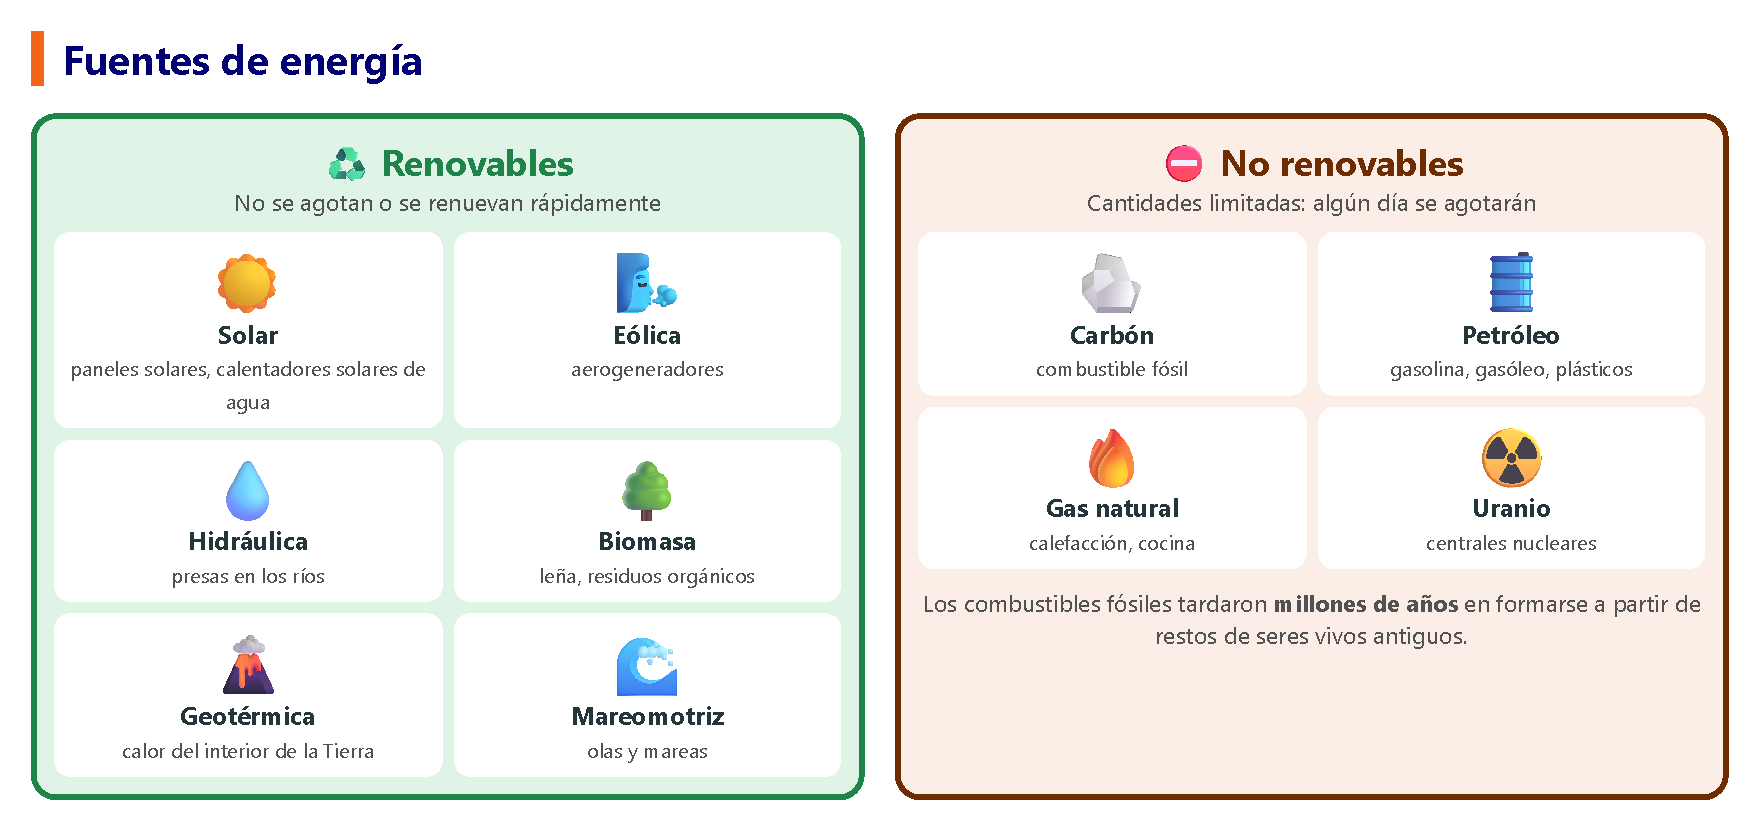
\includegraphics[width=\textwidth]{FigurasSVG/Unit_9_Energy/pdf/sources_es.pdf}
    \caption{Fuentes de energía renovables y no renovables.}
    \label{fig:u9_sources}
\end{figure}

\begin{impt}
    \negsubro{Uso directo o producción de electricidad}: una fuente de energía se puede aprovechar \textbf{directamente} (p.\ ej., quemar biomasa para calentarse o calentar agua con la luz del Sol) o usarse para \textbf{producir electricidad}, normalmente haciendo girar una turbina conectada a un generador (en las centrales hidroeléctricas, eólicas, solares, térmicas o nucleares).
\end{impt}

\begin{exercise}
    Clasifica estas fuentes de energía en renovables o no renovables, e indica si cada una se usa \textbf{directamente} o para \textbf{producir electricidad}: a) gas natural quemado en una central; b) leña quemada en una chimenea; c) luz del Sol en paneles solares que calientan agua directamente; d) uranio en una central nuclear.
    \begin{solu}
        \begin{enumerate}[label=\alph*)]
            \item No renovable; se usa para producir electricidad.
            \item Renovable (biomasa); se usa directamente.
            \item Renovable; se usa directamente (no se produce electricidad).
            \item No renovable; se usa para producir electricidad.
        \end{enumerate}
    \end{solu}
\end{exercise}

\subsection{La energía eólica en Castilla-La Mancha}

Castilla-La Mancha es una de las comunidades autónomas españolas con más parques eólicos, gracias a su terreno llano y a sus vientos fuertes y constantes. Un \negsubro{aerogenerador} transforma la \textbf{energía cinética} del viento en \textbf{energía eléctrica}: el viento hace girar las palas, que mueven un eje conectado a un generador.

\begin{figure}[H]
    \centering
    % [FIGURA ORIGINAL] \includegraphics[width=\textwidth]{Unit_9/wind_turbine}
    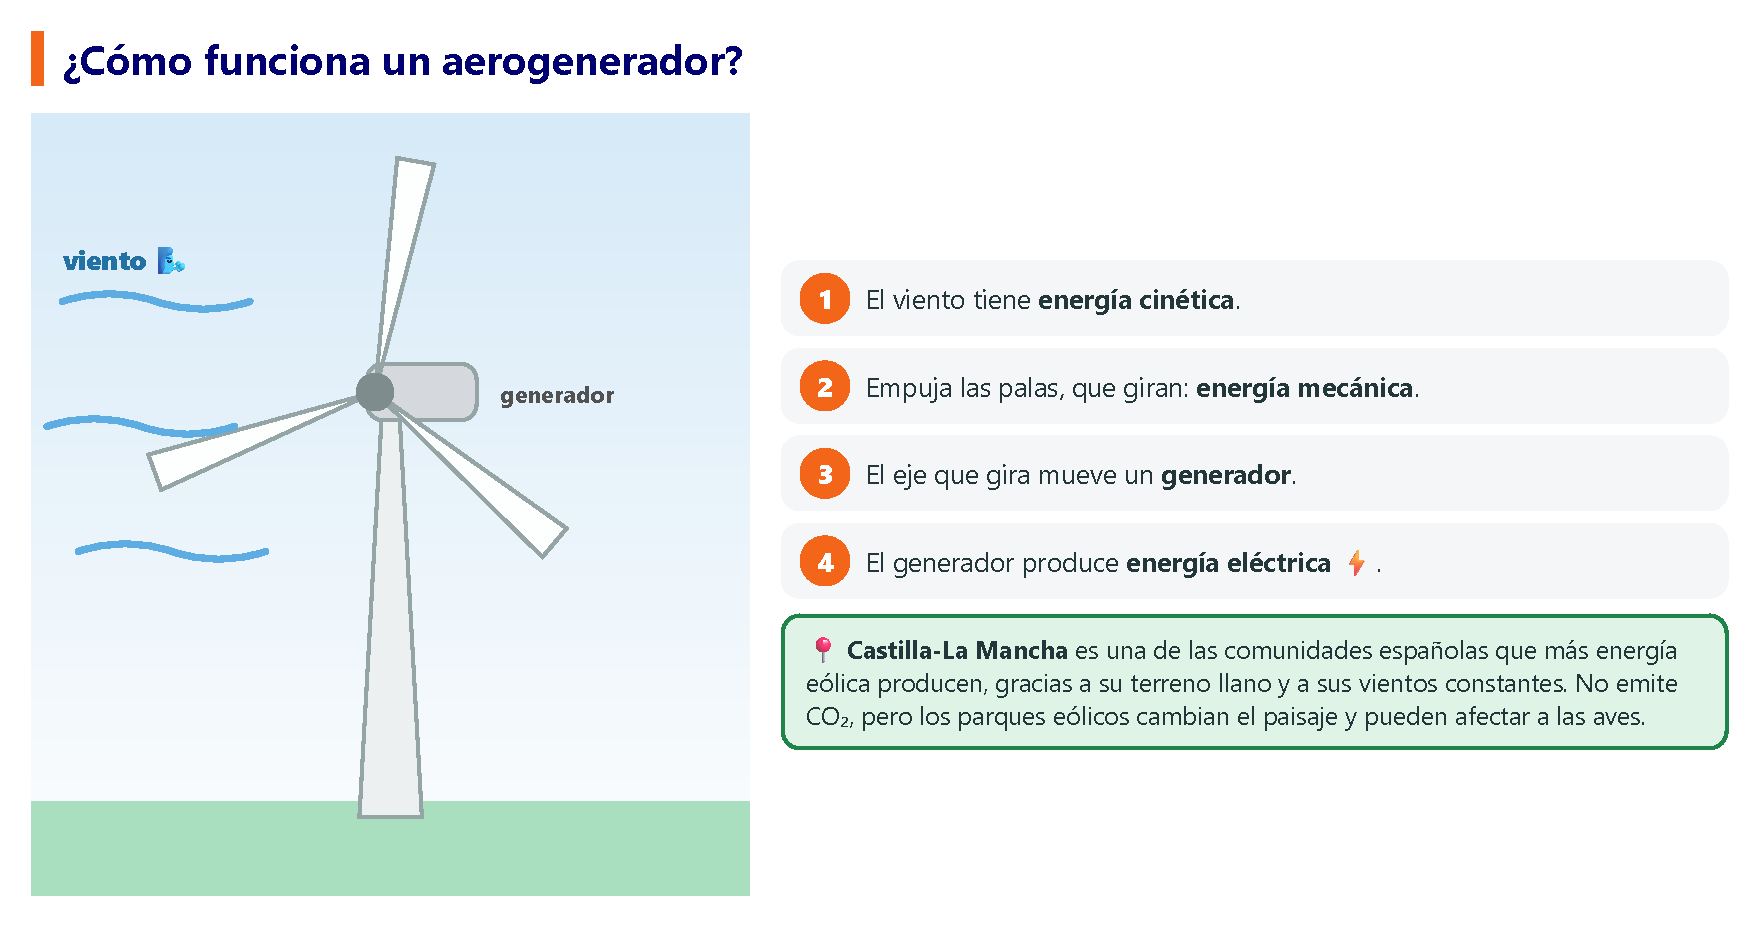
\includegraphics[width=\textwidth]{FigurasSVG/Unit_9_Energy/pdf/wind_turbine_es.pdf}
    \caption{Cómo transforma un aerogenerador la energía del viento en electricidad.}
    \label{fig:u9_wind_turbine}
\end{figure}

\begin{impt}
    \negsubro{La energía eólica en nuestra región}: la energía eólica es, junto con la solar, una de las principales fuentes renovables que se producen en Castilla-La Mancha, y la región es una de las mayores productoras de energía eólica de España. Así se obtiene una gran parte de la electricidad de la región sin emitir gases de efecto invernadero; aun así, los parques eólicos deben planificarse con cuidado, porque pueden afectar a las aves, a los murciélagos y al paisaje.
\end{impt}

\begin{exercise}
    Explica dos ventajas y un inconveniente de instalar parques eólicos en Castilla-La Mancha.
    \begin{solu}
        \textbf{Ventajas} (dos cualesquiera): el viento es un recurso renovable e inagotable; producir electricidad con el viento no emite \ch{CO2} ni otros contaminantes; la región tiene vientos fuertes y constantes, lo que la convierte en un lugar eficiente; reduce la dependencia de los combustibles fósiles importados. \\
        \textbf{Inconveniente} (uno cualquiera): los aerogeneradores cambian el paisaje; pueden afectar a las aves y a los murciélagos; la producción de electricidad depende de que sople el viento, así que no es constante.
    \end{solu}
\end{exercise}

\begin{exercise}
    Un aerogenerador de Castilla-La Mancha tiene una potencia nominal de \qty{2}{\mega\watt}. Si funciona a plena potencia durante \qty{8}{\hour} en un día, calcula la energía que produce ese día, en kWh y en MJ.
    \begin{solu}
        \(E = P \cdot t = \qty{2000}{\kilo\watt} \cdot \qty{8}{\hour} = \textbf{\num{16000} kWh}\). \\
        En MJ: \(\qty{16000}{\kwh} \cdot \qty{3.6e6}{\joule\per\kwh} = \qty{5.76e10}{\joule} = \textbf{\num{57600} MJ}\).
    \end{solu}
\end{exercise}

%\subsection{Electrical quantities}
%
%A generator produces an \textbf{electric current} (electric charges moving in an orderly way) inside an \textbf{electric circuit}.
%
%\begin{figure}[H]
%    \centering
%    \includegraphics[width=\textwidth]{Unit_9/circuit}
%    \caption{A simple electric circuit and the three electrical quantities.}
%    \label{fig:u9_circuit}
%\end{figure}
%
%\begin{exercise}
%    Name the basic parts of a simple electric circuit (battery, bulb) and explain the function of each one.
%    \begin{solu}
%        \textbf{Generator} (e.g.\ battery): produces the electric current. \\
%        \textbf{Wires/connectors}: made of a conductive material (e.g.\ copper); transport the current between components. \\
%        \textbf{Switch}: a control element that opens or closes the circuit, stopping or starting the current. \\
%        \textbf{Receiver} (e.g.\ bulb, motor): transforms the electric current into another form of energy (light, movement, etc.).
%    \end{solu}
%\end{exercise}
%
%
%\begin{exercise}
%    A charge of \qty{15}{\coulomb} flows through a wire in \qty{5}{\second}. Calculate the current intensity.
%    \begin{solu}
%        \(I = \dfrac{Q}{t} = \dfrac{\qty{15}{\coulomb}}{\qty{5}{\s}} = \textbf{3 A}\).
%    \end{solu}
%\end{exercise}
%
%\begin{exercise}
%    State which electrical quantity (current intensity, potential difference or resistance) is being described in each case: a) it is measured in volts; b) it opposes the flow of electric current; c) it is measured using an ammeter.
%    \begin{solu}
%        \begin{enumerate}[label=\alph*)]
%            \item Potential difference.
%            \item Resistance.
%            \item Current intensity.
%        \end{enumerate}
%    \end{solu}
%\end{exercise}

%\subsection{Ohm's law}
%
%\begin{impt}
%    \negsubro{Ohm's law} relates the three electrical quantities of a circuit:
%    \begin{equation*}
%        I = \dfrac{\Delta V}{R}
%    \end{equation*}
%    The current intensity through a conductor is directly proportional to the potential difference applied to it, and inversely proportional to its resistance.
%\end{impt}
%
%\begin{figure}[H]
%    \centering
%    \includegraphics[width=\textwidth]{Unit_9/ohm_law}
%    \caption{Ohm's law: the triangle helps us to isolate each quantity.}
%    \label{fig:u9_ohm_law}
%\end{figure}
%
%\begin{example}
%    \textbf{A bulb of resistance \qty{60}{\ohm} is connected to a \qty{12}{\volt} battery. What current flows through it?}
%    \begin{equation*}
%        I = \dfrac{\Delta V}{R} = \dfrac{\qty{12}{\volt}}{\qty{60}{\ohm}} = \textbf{0.2 A}
%    \end{equation*}
%\end{example}
%
%\begin{exercise}
%    A hairdryer connected to the \qty{230}{\volt} mains has a resistance of \qty{46}{\ohm}. Calculate the current intensity that flows through it.
%    \begin{solu}
%        \(I = \dfrac{\Delta V}{R} = \dfrac{\qty{230}{\volt}}{\qty{46}{\ohm}} = \textbf{5 A}\).
%    \end{solu}
%\end{exercise}
%
%\begin{exercise}
%    A current of \qty{0.5}{\ampere} flows through a resistor connected to a \qty{9}{\volt} battery. Calculate the resistance of the resistor.
%    \begin{solu}
%        From Ohm's law, \(R = \dfrac{\Delta V}{I} = \dfrac{\qty{9}{\volt}}{\qty{0.5}{\ampere}} = \textbf{18}\ \Omega\).
%    \end{solu}
%\end{exercise}
%
%\begin{exercise}
%    A resistor has a resistance of \qty{25}{\ohm}. What potential difference must be applied to it so that a current of \qty{2}{\ampere} flows through it?
%    \begin{solu}
%        From Ohm's law, \(\Delta V = I \cdot R = \qty{2}{\ampere} \cdot \qty{25}{\ohm} = \textbf{50 V}\).
%    \end{solu}
%\end{exercise}

%\subsection{Series and parallel circuits}
%
%\begin{figure}[H]
%    \centering
%    \includegraphics[width=\textwidth]{Unit_9/series_parallel}
%    \caption{Bulbs connected in series and in parallel.}
%    \label{fig:u9_series_parallel}
%\end{figure}
%
%\begin{example}
%    A string of old-style Christmas lights wired \textbf{in series} switches off completely if a single bulb breaks. Household electrical installations are wired \textbf{in parallel}: switching off one lamp, or a bulb breaking, does not switch off the other appliances connected to the mains.
%\end{example}
%
%
%\begin{exercise}
%    Say whether the bulbs in each situation are connected in series or in parallel, and justify your answer: a) when one bulb is unscrewed, all the other bulbs go off too; b) a fridge keeps working even if a lamp in another room is switched off.
%    \begin{solu}
%        \begin{enumerate}[label=\alph*)]
%            \item \textbf{Series}: there is a single path for the current, so removing one bulb interrupts the whole circuit.
%            \item \textbf{Parallel}: each appliance is on its own branch, so it works independently of the others.
%        \end{enumerate}
%    \end{solu}
%\end{exercise}
%
%\begin{exercise}
%    Three identical bulbs are connected \textbf{in series} to a \qty{12}{\volt} battery. If one bulb burns out, what happens to the other two? Explain.
%    \begin{solu}
%        In a series circuit there is only \textbf{one path} for the current. If one bulb burns out, it interrupts that path, so no current can flow anywhere in the circuit: the \textbf{other two bulbs also go off}.
%    \end{solu}
%\end{exercise}
%
%\begin{exercise}
%    Two lamps with different resistances are connected \textbf{in parallel} to the \qty{230}{\volt} mains supply. Explain why both lamps are subject to the same potential difference, and what this means for their brightness.
%    \begin{solu}
%        In a parallel circuit, every branch connects the same two points, so the potential difference across each branch equals the source voltage: both lamps have \qty{230}{\volt} across them. However, by Ohm's law (\(I = \Delta V / R\)), the lamp with the \textbf{lower resistance} draws a \textbf{higher current}, so it will shine \textbf{brighter}, even though both receive the same potential difference.
%    \end{solu}
%\end{exercise}

%----------------------------------------------------------------------------------------

\section{El impacto ambiental de la energía}

Obtener, transportar y usar la energía tiene consecuencias para el medio ambiente: se agotan los recursos, se generan residuos tóxicos y se contaminan el aire, el agua y el suelo.

\begin{itemize}
    \item \negsubro{Lluvia ácida}: al quemar combustibles fósiles, las sustancias que se liberan se combinan con el agua de lluvia; esta lluvia daña las plantas y puede afectar a zonas muy alejadas del lugar donde se produjo la contaminación.
    \item \negsubro{Calentamiento global}: la quema de combustibles fósiles aumenta el dióxido de carbono de la atmósfera, lo que intensifica el efecto invernadero natural y eleva la temperatura media del planeta.
\end{itemize}

\begin{table}[H]
    \centering
    \begin{tabular}{p{5.3cm}p{5.3cm}}
        \toprule
        \textbf{Fuentes renovables} & \textbf{Fuentes no renovables} \\
        \midrule
        No emiten sustancias perjudiciales, pero pueden alterar mucho el paisaje y los hábitats de los seres vivos (p.\ ej., los aerogeneradores o las grandes centrales solares o hidroeléctricas). &
        Los combustibles fósiles emiten \ch{CO2} y otros gases de efecto invernadero, y provocan lluvia ácida; su extracción modifica el terreno, y los vertidos accidentales contaminan. Los materiales radiactivos generan residuos peligrosos que hay que almacenar de forma segura. \\
        \bottomrule
    \end{tabular}
    \caption{Impacto ambiental de las fuentes de energía renovables y no renovables.}
    \label{tab:u9_impact}
\end{table}

\begin{exercise}
    Relaciona cada causa con su consecuencia para el medio ambiente: a) quemar combustibles fósiles en el transporte; b) un accidente de un petrolero; c) los residuos radiactivos de una central nuclear. \newline
    Consecuencias: 1. grandes vertidos de petróleo; 2. contaminación del aire / calentamiento global; 3. necesidad de almacenar residuos peligrosos durante mucho tiempo.
    \begin{solu}
        a) \(\to\) 2; \quad b) \(\to\) 1; \quad c) \(\to\) 3.
    \end{solu}
\end{exercise}

\begin{exercise}
    Explica cómo contribuye la quema de combustibles fósiles a dos problemas ambientales distintos de los estudiados en esta unidad.
    \begin{solu}
        La quema de combustibles fósiles libera \ch{CO2}, que intensifica el \textbf{efecto invernadero} natural y provoca el \textbf{calentamiento global}. También libera óxidos de azufre y de nitrógeno, que se combinan con el agua de la atmósfera y caen como \textbf{lluvia ácida}, que daña las plantas y los ecosistemas, a veces lejos del lugar donde se produjo la contaminación.
    \end{solu}
\end{exercise}

%----------------------------------------------------------------------------------------

\section{La energía que usamos}

\begin{itemize}
    \item \negsubro{Energía primaria}: la que se obtiene directamente de una fuente de la naturaleza (p.\ ej., la energía química del carbón o la energía cinética del viento), y que se usa directamente o se transforma.
    \item \negsubro{Energía final}: la que realmente llega al consumidor y este utiliza (p.\ ej., la electricidad o la gasolina), después de haberse transformado y transportado.
\end{itemize}

\begin{impt}
    Un país que consume más energía de la que produce es un \negsubro{importador de energía}; un país que produce más de la que consume es un \negsubro{exportador de energía}.
\end{impt}

La figura~\ref{fig:u9_energy_mix} muestra cómo se repartió en 2021 el consumo mundial de energía según la fuente primaria; la usarás en el ejercicio siguiente.

\begin{figure}[H]
    \centering
    % [FIGURA ORIGINAL] \includegraphics[width=0.95\textwidth]{Unit_9/energy_mix}
    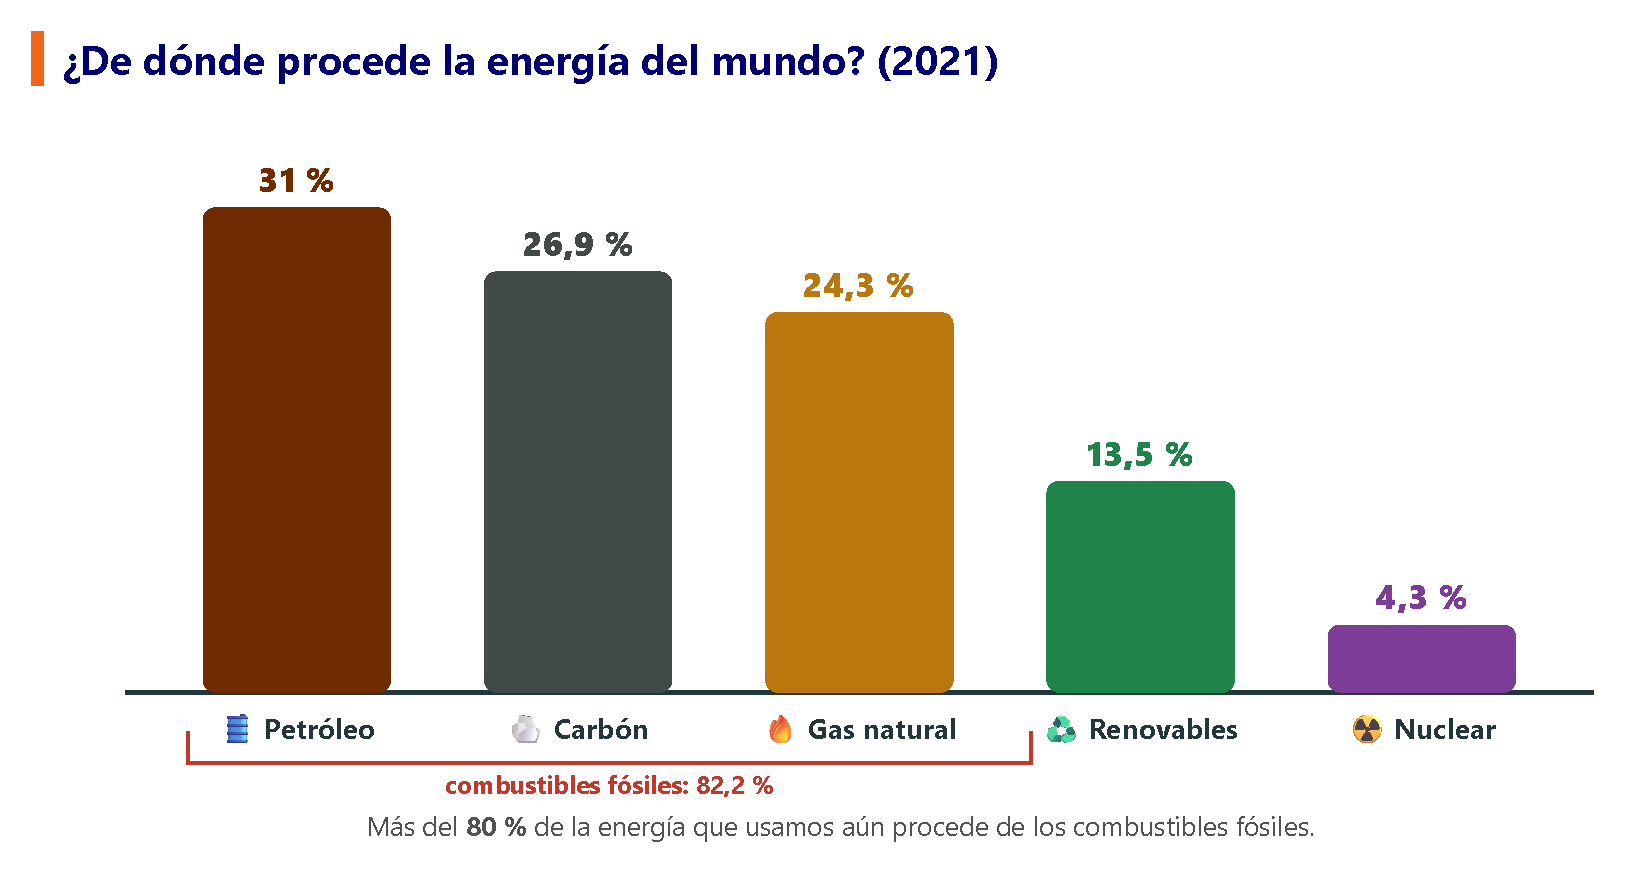
\includegraphics[width=0.95\textwidth]{FigurasSVG/Unit_9_Energy/pdf/energy_mix_es.pdf}
    \caption{Consumo mundial de energía primaria según la fuente, 2021.}
    \label{fig:u9_energy_mix}
\end{figure}

\begin{exercise}
    En 2021, el consumo total de energía en el mundo se repartió así según la fuente primaria: petróleo 31\,\%, gas natural \num{24.3}\,\%, carbón \num{26.9}\,\%, nuclear \num{4.3}\,\% y renovables \num{13.5}\,\%, de un total de \num{14220} Mtep (millones de toneladas equivalentes de petróleo). Calcula la energía, en Mtep, que se consumió procedente del petróleo y de las renovables.
    \begin{solu}
        Petróleo: \(\num{14220} \cdot \dfrac{31}{100} \approx \num{4408.2}\) Mtep. \\
        Renovables: \(\num{14220} \cdot \dfrac{\num{13.5}}{100} \approx \num{1919.7}\) Mtep.
    \end{solu}
\end{exercise}

\begin{exercise}
    Explica por qué la energía eléctrica aparece en el consumo de energía \textbf{final} de un país, pero no directamente en su consumo de energía \textbf{primaria}.
    \begin{solu}
        La electricidad no es en sí misma una fuente de energía primaria: se produce transformando fuentes primarias (combustibles fósiles, nuclear, viento, agua, Sol, etc.). Una vez producida, se cuenta como energía \textbf{final}, ya que es la que realmente llega al consumidor y este utiliza.
    \end{solu}
\end{exercise}

\begin{exercise}
    Un país produjo 145 Mtep de energía primaria en un año, pero consumió 165 Mtep. ¿Fue ese año un país importador o exportador de energía? Justifica tu respuesta y calcula el déficit energético, en Mtep.
    \begin{solu}
        Como el consumo (165 Mtep) es mayor que la producción (145 Mtep), ese año el país fue \textbf{importador de energía}: tuvo que traer energía del extranjero para cubrir sus necesidades. \\
        Déficit \(= 165 - 145 = \textbf{20 Mtep}\).
    \end{solu}
\end{exercise}

%----------------------------------------------------------------------------------------

\section{Ahorro energético y desarrollo sostenible}

\begin{definition}[Desarrollo sostenible]
    Desarrollo que cubre las necesidades de energía actuales sin malgastar recursos ni causar daños innecesarios al medio ambiente, de modo que las generaciones futuras también puedan cubrir las suyas.
\end{definition}

\begin{itemize}
    \item \negsubro{Diseño de productos y edificios eficientes}: vehículos y electrodomésticos de bajo consumo; casas bien aisladas para evitar pérdidas de energía.
    \item \negsubro{Fuentes de energía locales}: instalar paneles solares; aprovechar el curso natural de los ríos; usar como biomasa los residuos orgánicos de la zona.
    \item \negsubro{Evitar el consumo innecesario}: usar el transporte público; comprar solo lo necesario; consumir productos locales.
    \item \negsubro{En casa}: usar bombillas de bajo consumo; apagar las luces y los aparatos que no se estén usando; usar la calefacción y el aire acondicionado con sensatez; no desperdiciar el agua caliente.
\end{itemize}

\begin{figure}[H]
    \centering
    % [FIGURA ORIGINAL] \includegraphics[width=\textwidth]{Unit_9/energy_saving}
    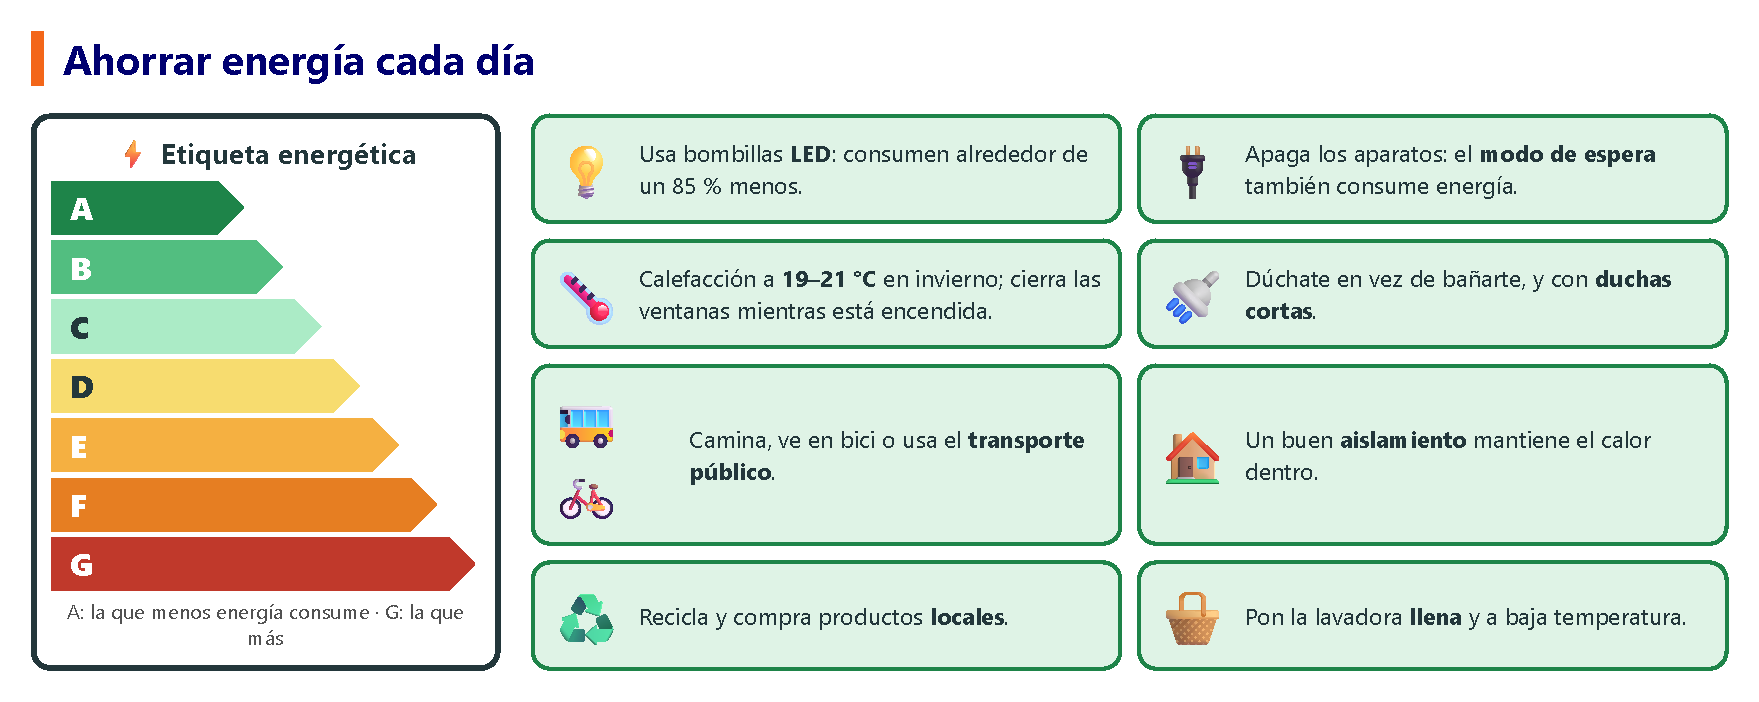
\includegraphics[width=\textwidth]{FigurasSVG/Unit_9_Energy/pdf/energy_saving_es.pdf}
    \caption{La etiqueta energética y algunas formas sencillas de ahorrar energía.}
    \label{fig:u9_energy_saving}
\end{figure}

\begin{exercise}
    Un frigorífico de clase D (consumo medio) gasta \qty{600}{\kwh} al año. Los frigoríficos de clase A consumen alrededor de un 55\,\% \textbf{menos} que la media, y los de clase G, alrededor de un 125\,\% \textbf{más} que la media.
    \begin{enumerate}[label=\letraminuscula]
        \item ¿Cuánto consumiría al año un frigorífico de clase A?
        \item ¿Cuánto consumiría al año un frigorífico de clase G?
    \end{enumerate}
    \begin{solu}
        \begin{enumerate}[label=\alph*)]
            \item \(\qty{600}{\kwh} \cdot (1 - \num{0.55}) = 600 \cdot \num{0.45} = \qty{270}{\kwh}\) al año.
            \item \(\qty{600}{\kwh} \cdot (1 + \num{1.25}) = 600 \cdot \num{2.25} = \qty{1350}{\kwh}\) al año.
        \end{enumerate}
    \end{solu}
\end{exercise}

\begin{exercise}
    Decide si cada acción ahorra energía y explica por qué: a) desenchufar los aparatos eléctricos que no se están usando; b) abrir las ventanas en invierno para ventilar mientras la calefacción está encendida; c) usar bombillas de bajo consumo.
    \begin{solu}
        \begin{enumerate}[label=\alph*)]
            \item \textbf{Ahorra energía}: muchos aparatos siguen consumiendo un poco de electricidad en modo de espera.
            \item \textbf{No ahorra energía} (si se hace con la calefacción encendida): el calor se escapa y la calefacción tiene que trabajar más para compensarlo. (Ventilar un rato con la calefacción \textit{apagada} sí está bien).
            \item \textbf{Ahorra energía}: las bombillas LED o de bajo consumo convierten en luz un porcentaje mayor de la energía eléctrica y desperdician menos en forma de calor, es decir, degradan menos energía.
        \end{enumerate}
    \end{solu}
\end{exercise}

\begin{exercise}
    Una familia cambia 10 bombillas incandescentes (de \qty{60}{\watt} cada una) por 10 bombillas LED (de \qty{9}{\watt} cada una), que usa una media de \qty{4}{\hour} al día. Calcula la energía que ahorra cada día, en kWh.
    \begin{solu}
        Bombillas incandescentes: \(10 \cdot \qty{60}{\watt} = \qty{600}{\watt} = \qty{0.6}{\kilo\watt}\); \(\qty{0.6}{\kilo\watt} \cdot \qty{4}{\hour} = \qty{2.4}{\kwh}\). \\
        Bombillas LED: \(10 \cdot \qty{9}{\watt} = \qty{90}{\watt} = \qty{0.09}{\kilo\watt}\); \(\qty{0.09}{\kilo\watt} \cdot \qty{4}{\hour} = \qty{0.36}{\kwh}\). \\
        Energía ahorrada \(= \num{2.4} - \num{0.36} = \textbf{\num{2.04} kWh al día}\).
    \end{solu}
\end{exercise}

%----------------------------------------------------------------------------------------

\section*{Resumen}

\begin{itemize}
    \item \textbf{Energía}: capacidad de un cuerpo para producir cambios; se mide en julios (también en kJ, cal, kWh, tep).
    \item \textbf{Formas de energía}: cinética, potencial (gravitatoria y elástica), mecánica, térmica, eléctrica, radiante, química y nuclear.
    \item \textbf{Propiedades}: la energía se puede transferir, almacenar, transportar y transformar; siempre se conserva (en total), pero una parte se degrada (se convierte en calor no aprovechable) cada vez que se transforma.
    \item \textbf{Efectos del calor}: el calor específico \(c\) mide el calor necesario para elevar \qty{1}{\celsius} la temperatura de \qty{1}{\kg} de una sustancia (\(Q = mc\Delta T\)); la mayoría de las sustancias se dilatan al calentarse y se contraen al enfriarse (dilatación térmica).
    \item \textbf{Fuentes de energía}: las renovables (viento, agua, Sol, biomasa, geotérmica) no se agotan; las no renovables (combustibles fósiles, materiales radiactivos) son limitadas y acabarán agotándose. La energía eólica es una de las principales fuentes renovables que se producen en Castilla-La Mancha.
%    \item \textbf{Electrical quantities}: current intensity \(I\) (A), potential difference \(\Delta V\) (V) and resistance \(R\) (\(\Omega\)), related by \textbf{Ohm's law}, \(I = \Delta V / R\). Circuits can be wired in \textbf{series} (single path) or in \textbf{parallel} (independent branches).
    \item \textbf{Impacto ambiental}: la quema de combustibles fósiles provoca lluvia ácida y calentamiento global; todas las fuentes de energía tienen algún impacto sobre el paisaje o los hábitats.
    \item \textbf{Energía primaria y energía final}: la energía primaria procede directamente de una fuente; la energía final es la que realmente llega al consumidor y este utiliza (p.\ ej., la electricidad).
    \item \textbf{Desarrollo sostenible}: ahorrar energía y usar recursos eficientes, locales y renovables para cubrir nuestras necesidades sin poner en peligro a las generaciones futuras.
\end{itemize}

\section{Vocabulario}

\begin{vocabulary}[Energía (\textit{energy})]
    Magnitud física que mide la capacidad que tiene un cuerpo para producir cambios en sí mismo o en otros cuerpos.
\end{vocabulary}

\begin{vocabulary}[Energía cinética (\textit{kinetic energy})]
    Energía que tiene un cuerpo por estar en movimiento.
\end{vocabulary}

\begin{vocabulary}[Energía potencial (\textit{potential energy})]
    Energía que tiene un cuerpo por su posición o su estado (p.\ ej., por su altura o por estar estirado).
\end{vocabulary}

\begin{vocabulary}[Fuente de energía (\textit{energy source})]
    Cualquier material o recurso natural del que se puede obtener energía aprovechable.
\end{vocabulary}

\begin{vocabulary}[Renovable (\textit{renewable})]
    Fuente de energía cuyos recursos se pueden reponer después de usarlos, o que nunca se agotan.
\end{vocabulary}

\begin{vocabulary}[No renovable (\textit{non-renewable})]
    Fuente de energía cuyos recursos son limitados y no se pueden reponer una vez consumidos.
\end{vocabulary}

\begin{vocabulary}[Corriente eléctrica (\textit{electric current})]
    Movimiento ordenado de cargas eléctricas a través de un conductor.
\end{vocabulary}

\begin{vocabulary}[Calor específico (\textit{specific heat capacity})]
    Cantidad de calor necesaria para elevar \qty{1}{\celsius} la temperatura de \qty{1}{\kg} de una sustancia.
\end{vocabulary}

\begin{vocabulary}[Dilatación térmica (\textit{thermal expansion})]
    Aumento de volumen de una sustancia cuando sube su temperatura.
\end{vocabulary}

\begin{vocabulary}[Energía eólica (\textit{wind energy})]
    Energía cinética del viento, que se aprovecha directamente o se transforma en energía eléctrica mediante aerogeneradores.
\end{vocabulary}

\begin{vocabulary}[Ley de Ohm (\textit{Ohm's law})]
    Relación entre la intensidad de corriente, la diferencia de potencial y la resistencia en un circuito: \(I = \Delta V / R\).
\end{vocabulary}

\begin{vocabulary}[Circuito en serie (\textit{series circuit})]
    Circuito en el que los componentes están conectados uno detrás de otro, en un único camino.
\end{vocabulary}

\begin{vocabulary}[Circuito en paralelo (\textit{parallel circuit})]
    Circuito en el que los componentes están conectados en ramas distintas entre los mismos dos puntos.
\end{vocabulary}

\begin{vocabulary}[Degradación de la energía (\textit{energy degradation})]
    Pérdida, en cualquier transformación de la energía, de una parte de ella en forma de calor no aprovechable.
\end{vocabulary}

\begin{vocabulary}[Energía primaria (\textit{primary energy})]
    Energía que se obtiene directamente de una fuente natural.
\end{vocabulary}

\begin{vocabulary}[Energía final (\textit{final energy})]
    Energía que realmente llega al consumidor y que este utiliza.
\end{vocabulary}

\begin{vocabulary}[Desarrollo sostenible (\textit{sustainable development})]
    Desarrollo que cubre las necesidades actuales sin poner en peligro la capacidad de las generaciones futuras para cubrir las suyas.
\end{vocabulary}
